\documentclass[11pt]{article}
\usepackage{amsmath,textcomp,amssymb,geometry,graphicx,enumerate}
\usepackage{tabu}
\usepackage{algorithm} % Boxes/formatting around algorithms
\usepackage[noend]{algpseudocode} % Algorithms
\usepackage{graphicx}
\usepackage{caption}
\usepackage{subcaption}
\usepackage{siunitx}

\def\Name{Sam Holladay}  % Your name
\def\SID{24194437}  % Your student ID number
\def\Homework{8} % Number of Homework
\def\Session{Fall 2015}


\title{EE230C Final Project: Monolayer Graphene}
\author{Sam Holladay, Saavan Patel, and Charles Zhang}
\markboth{EE230C-Holladay, Patel, and Zhang}{EE230C-Holladay, Patel, and Zhang}
\pagestyle{myheadings}
\date{}

\newenvironment{qparts}{\begin{enumerate}[{(}a{)}]}{\end{enumerate}}
\def\endproofmark{$\Box$}
\newenvironment{proof}{\par{\bf Proof}:}{\endproofmark\smallskip}

\textheight=9in
\textwidth=6.5in
\topmargin=-.75in
\oddsidemargin=0.25in
\evensidemargin=0.25in


\begin{document}
\maketitle

\section*{i.} The experimental performance of several sub-100 nm graphene transistors were demonstrated by Wu for RF purposes\cite{wu2010}. The topology of these graphene devices is shown in Figure 1. The current-voltage characteristics of the 70 nm FETs were measured at both room temperature and low temperature. The performance of the FETs were also modeled, and Figure 2a and 2b shows a comparison of the experimental and modeled current $I_d$ vs the gate voltage $V_g$ and the drain voltage $V_d$, respectively. 
\begin{figure}[h!]
\centering 
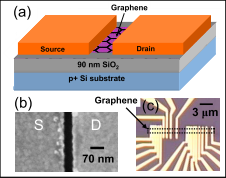
\includegraphics[width=0.5\textwidth]{paper1_fet.png}
\caption{(a) Schematic view of Wu's back-gated graphene FET, (b) SEM image of metal contacts of a 70nm device and (c) optical image of the fabricated devices.}\label{fig:FET}
\end{figure}

Experimental data of the contact resistance was also collected at different temperatures, as seen in Figure 3. For the 70 nm device, contact resistance for electrons was around 275 $~\Omega -\mu$m. Mobility data vs temperature was also collected, shown in Figure 4.

\begin{figure}[h!]
\centering 
\begin{subfigure}[b]{0.3\textwidth}
        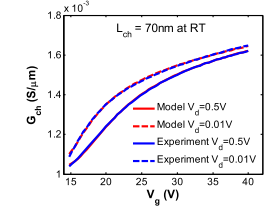
\includegraphics[width=\textwidth]{paper1_idvg3.png}
        \caption{Comparison of experiment and model of the transfer characteristics.}
        \label{fig:Idvg}
\end{subfigure}
\begin{subfigure}[b]{0.3\textwidth}
        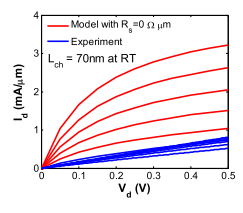
\includegraphics[width=\textwidth]{paper1_idvd3.png}
        \caption{Modeled output characteristics with $R_s=0$ vs experiment.}
        \label{fig:Idvd}
\end{subfigure}
\caption{Measurements by Wu of 70 nm device at room temperature}\label{fig:animals}
\end{figure}

\begin{figure}[h!]
\centering 
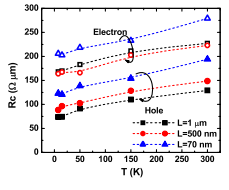
\includegraphics[width=0.4\textwidth]{paper1_contactres.png}
\caption{Contact resistance $R_c$ vs T from devices with different channel length, from 1 $\mu$m to 70 nm.}\label{fig:FET}
\end{figure}

\begin{figure}[h!]
\centering 
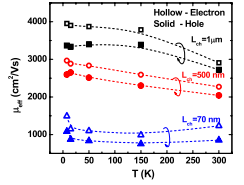
\includegraphics[width=0.4\textwidth]{paper1_mobilitydata.png}
\caption{Effective electron and hole mobility $\mu_{eff}$ vs T from devices with different channel length, from 1 $\mu$m to 70 nm.}\label{fig:FET}
\end{figure}

Additionally, in 2011 Meric et al \cite{meric2011} took a comprehensive look at channel-length scaling of graphene FETs, including several with channel lengths under 100 nm. Their graphene FET design is similar to Wu's, and is shown in Figure 5.

\section*{ii.} To calculate the current-voltage characteristics, the bandstructure of graphene must be derived. The Hamiltonian matrix is first constructed, and the eigenvalues are determined computationally. Using the method of Linear Combination of Atomic Orbitals as described in Slater and Koster \cite{slaterkoster1954}, we construct the on and off diagonal terms Hamiltonians. A six-band tight-binding model is used, which includes the $p_z,d_{yz}, d_{zx}$ orbitals. These have binding energies described by Boykin \cite{boykin2011}. The band structure is generated by finding the eigenvalues of the 6x6 Hamiltonian generated by the equation:

$H = H_{on} + H_{off}e^{i\vec{k}\vec{t_1}} + H^T_{off}e^{-i\vec{k}\vec{t_1}} + H_{off}e^{i\vec{k}\vec{t_2}} + H^T_{off}e^{-i\vec{k}\vec{t_2}}$

Here, the vectors $\vec{t_1}$ and $\vec{t_2}$ represent the basis vectors for the graphene unit cell, as denoted in Figure 5. The $\vec{k}$ is the momentum vector, which we allow to take values over the entire first Brillouin zone. 

\begin{figure}[h!]
\centering
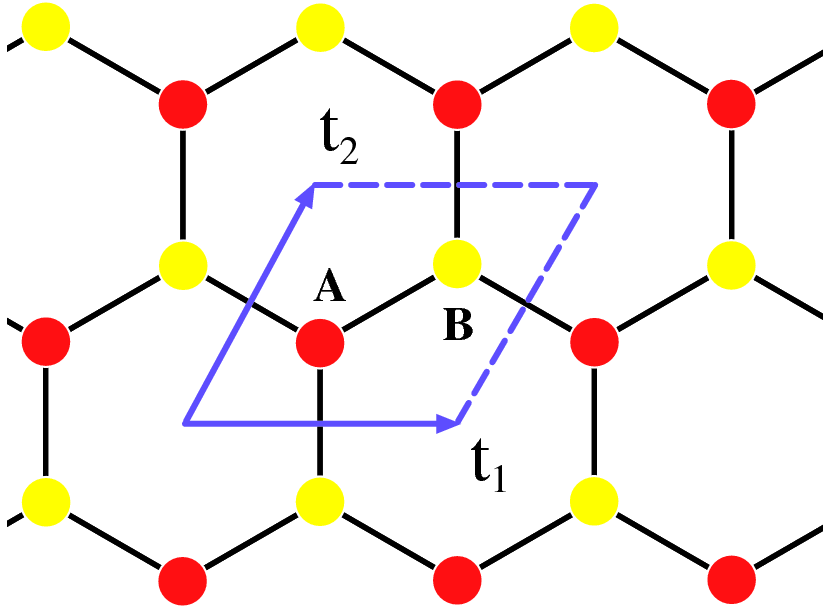
\includegraphics[width=0.4\textwidth]{graphene_unit_cell.png}
\caption{The Graphene Unit Cell, with translation vectors. Different colors represent the different atoms in the unit cell}
\end{figure}

The bandstructure is presented in Figure 6.

\begin{figure}[h!]
\centering
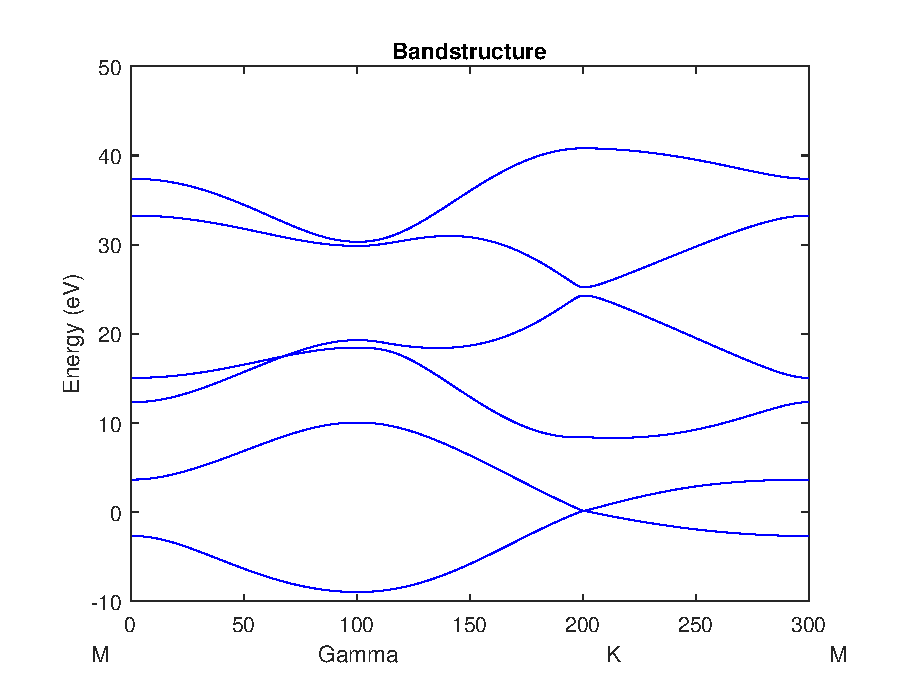
\includegraphics[width=0.4\textwidth]{Bandstructure.eps}
\caption{Dispersion relation using 6-band tight binding model}
\end{figure}

To derive the current-voltage characteristics of the transistor, we proceed from the fundamental quasi-ballistic equation for current:

$$I_d = -ew(\sum_{k_x>0, ky}f_{k}v_{k} - \sum_{k_x<0, ky}f_{k}v_{k})$$

This includes back-scattering of electrons going back over the barrier from the drain. We recall the expressions for $f_{k}$ and $v_{k}$:

$$f_{k}=\frac{1}{1+exp(\frac{\mathcal{E}_{k}(k_x,k_y) - \mu}{k_BT})}, \hspace{1em} v_{k} = \frac{1}{\hbar}\nabla_k(E)= \frac{1}{\hbar}(\frac{dE}{dk_x}+\frac{dE}{dk_y})$$

Here, since we are working from the numerical values of the rigorous bandstructure, $v_k$ is calculated numerically from the gradient of $E_k$ with respect to both $k_x$ and $k_y$. Analytic approximations for band structure are shown below, in section iii.

After deriving the bandstructure, the current can be determined computationally after converting the sum into a double integral by taking the limit of $k_x$ and $k_y$ to 0 and normalizing by $\frac{1}{4\pi^2}$:

$$\sum_{k_x>0, ky}f_{k}v_{k} =\int_{0}^{\infty}dk_xdk_yv_{k}f_{k} = \int_{0}^{\infty}\frac{1}{4\pi^2}dk_xdk_y\frac{1}{1+exp(\frac{\mathcal{E}_{k} - \mu_S}{k_BT})}\frac{1}{\hbar}\nabla_k(E)$$

With the corresponding expression for current from electrons going back over the barrier:

$$\sum_{k_x<0, ky}f_{k}v_{k} =\int_{-\infty}^{0}dk_xdk_yv_{k}f_{k} = \int_{-\infty}^{0}\frac{1}{4\pi^2}dk_xdk_y\frac{1}{1+exp(\frac{\mathcal{E}_{k} - \mu_D}{k_BT})}\frac{1}{\hbar}\nabla_k(E)$$

This takes care of current from electrons. To derive the total current, the hole current must also be taken into account, using the similar formula

$$I_{D-holes} = 2ew(\sum_{k_x<0, ky}f_{k}v_{k} - \sum_{k_x>0, ky}f_{k}v_{k})$$

because holes flow the opposite direction of electrons. While the velocity $v_k$ is calculated the same for holes, the Fermi function $f_k$ changes:

$$f_{kholes}=1-f_{kelectrons}$$

Then, proceeding the same way, the hole current is calculated and the total current $I_d$ is

$$I_d = I_{delectrons}+I_{dholes}$$

Thus a quasi-ballistic current dependent on the drain voltage $I_d$ is determined, with contact resistance not yet taken into account. This current is shown in Figure SOMETHING, and compares well to the similar measurements from Wu, seen in Figure 2b.


This, however, only takes care of variation with the drain voltage $V_d$. To implement gate control by the gate voltage $V_g$, the potential at the top of the barrier between source and drain is self-consistently with the number of carriers at the top of the barrier. For this model, charges in the channel are provided through thermionic emission from the source and drain contacts. Both electron and hole charges are taken into account to explain both positive and negative bias behavior. 

At equilibrium the concentration of carriers is the following:
$$N0 = \int_{-\infty}^{\infty}{D(E)f(E-Ef)dE}$$
where $D(E)$ is the density of states calculated from the band structure, and $f(E)$ is the fermi function at that energy level. This is used as an initial guess for the self consistent solution. We use the following equations, as described by \cite{ballistic2002}. 

\begin{enumerate}
\item $U_{TOB} = q\phi(\frac{C_G}{C_T} + \frac{C_D}{C_T}) + q^2\frac{N-N_0}{C_t}$ 
\item $N = \int_{-\infty}^{\infty}{D(E)f(E+U_{TOB}-\mu_s)} + \int_{-\infty}^{\infty}{D(E)f(E+U_{TOB}-\mu_d)}$
\end{enumerate}

The contribution for holes in the total carrier is added by substituting the Fermi functions and energies as described above. During all further models, we approximate that the source side potential, $\mu_s$, is grounded, and all other potentials are referenced from that point ($\mu_d$, $\mu_g$, etc.), making $\mu_s = 0$. 

For calculation of the gate capacitance, we calculate capacitances based on a 90nm SiO2 structure as described in by \cite{wu2010}. The drain to channel coupling capacitance is left as a fitting parameter, and is used to approximate the effects of DIBL and other short channel effects. 

**Figure showing DIBL plots***

Finally, contact resistance must be taken into account to obtain a final model for the current-voltage characteristics. Contact resistance values were taken from Wu's experimental results, and were both distinct for holes and electrons and dependent on channel length. As usual, the temperature was taken to be 300 K.

\section*{iii.} The injection velocity is defined as follows:

$$v_{inj} = \frac{\sum_{k_x>0, ky}f_{k}v_{k}}{\sum_{k_x>0, ky}f_{k}}$$

As before, this expression can be converted into an integral expression which includes $E_k$, when determining the Fermi function $f_{k}$, and $\nabla_k(E)$, when determining the velocity $v_{k}$.  Computing the integral as before using the rigorous bandstructure determined computationally, the injection velocity can be calculated as a function of $V_d$.

Graphene is notable because, due to the non-parabolic shape of its bandstructure, one cannot obtain an effective mass\cite{ariel2012} using the conventional definition $m^{*} = \hbar^2(\frac{d^2E(k)}{dk^2})^{-1}$. Instead we proceed with an alternative definition $m^{*} = \hbar^2k(\frac{dE(k)}{dk})^{-1}$. This is based on the linear bandstructure of graphene in a small region around the Dirac point. Using the usual effective mass approximation that $E=\frac{\hbar^2k_x^2}{2m^{*}}$. We set the fermi velocity of graphene to $v_f = 10^6 m/s$ as extracted from the band structure previously. From this point, we can derive the forward and backward scattering components of current as follows. 

$$I = -2ew[\sum_{kx>0,ky}{f_kv_k} - \sum_{kx<0,ky}{f_kv_k}]$$
\vspace{1em}



\section*{iv.}

\section*{v.}

\section*{Efficacy of device}

\begin{thebibliography}{9}

\bibitem{wu2010}
  Wu, Y.Q. et al.,
  \textit{"RF Performance of Short Channel Graphene FET"}.
  Tech. Dig Int. Electron Devices Meeting,
  pp 226-228,
  2010.
  
\bibitem{meric2011}
  Meric, I. et al.,
  \textit{"Channel Length Scaling in Graphene Field-Effect Transistors Studied with Pulsed Current-Voltage Measurements"}.
  Nano Letters 11 (3),
  1093-1097,
  (2011).
  
  \bibitem{boykin2011}
  Boykin, T. et al.,
  \textit{"Accurate six-band nearest-neighbor tight-binding model for the $\pi$ bands of bulk graphene and graphene nanoribbons."}.
  Journal of Applied Physics,
  109.10,
  (2011).
  
    \bibitem{ariel2012}
  Ariel, V. and A. Natan,
  \textit{"Electron Effective Mass in Graphene."}.
  arXiv:1206.6100,
  (2012).
  
  \bibitem{ballistic2002}
  Rahman, A. et. al.,
  \textit{"Theory of Ballistic Nanotransistors"}.
   IEEE Transactions on Electron Devices:50.9,
   1853-1864,
    (2003).
    
  \bibitem{slaterkoster1954}
  Slater, J.C., and G.F. Koster.,
  \textit{"Simplified LCAO method for the periodic potential problem."}.
   Physical Review 94.6,
    (1954): 1498.
    
  \bibitem{meric2008}
  Meric, I. et al.,
  \textit{"Current saturation in zero-bandgap, top-gated graphene field-effect transistors."}.
   Nature Nanotechnology 3 (11),
  654-659,
  (2008).
  
  \bibitem{chauhan2011}
  Chauhan, J. and J. Guo.,
  \textit{"Inelastic phonon scattering in graphene FETs."}.
   IEEE Transactions on Electron Devices 58 (11),
  3997-4003,
  (2011).
  
\end{thebibliography}


\end{document}
